\documentclass[12pt,a4paper]{article}
\usepackage[utf8]{inputenc}
\usepackage[german]{babel}
\usepackage[T1]{fontenc}
\usepackage{amsmath}
\usepackage{amsfonts}
\usepackage{amssymb}
\usepackage{graphicx}
\usepackage[left=2cm,right=2cm,top=2cm,bottom=2cm]{geometry}
\author{Tim}

\begin{document}
\newpage
\tableofcontents
\newpage

\section{Versuchsbeschreibung}
Ziel des Versuches ist die Vermessung der Dampfdruckkurve und die Bestimmung der Verdampfungsenthalpie von Wasser.\\

\subsection{Dampfdruckkurve}
In diesem Versuch soll nur der Übergang zwischen dem flüssigen und gasförmigen Aggregatzustand betrachtet werden. \\
In einer Flüssigkeit in einem evakuiertem, abgeschlossenem Gefäß verdampfen und kondensieren die Moleküle bis sich ein Gleichgewicht einstellt. Der Druck des Dampfes ist von der Temperatur und der Flüssigkeit abhängig und wird als Dampfdruck oder Sättigungsdruck bezeichnet. Der Zusammenhang von Sättigungsdampfdruck und Temperatur wird als Dampfdruckkurve bezeichnet. Wäre das Gefäß nicht evakuiert, würde sich das Gleichgewicht langsamer einstellen, der Dampfdruck wäre allerdings der gleiche, da die Partialdrücke einzelner Gase von der Anwesenheit anderer Gase nicht beeinflusst werden.

\subsection{Verdampfungsenthalpie}
Die Verdampfungsenthalpie beschreibt, wie viel Energie notwendig ist, um ein Mol des jeweiligen Stoffs (in diesem Fall Wasser) zu Verdampfen. Führt man einer gewissen Menge flüssigem Wasser langsam immer mehr Wärmeenergie zu und misst dabei die Temperatur, so ist die Verdampfungsenthalpie als Plateau beobachtbar. Trotz des Zuführens weiterer Wärmeenergie ändert sich die Temperatur nicht. \\

Der Sättigungsdampfdruck wird quantitativ durch die Clausius-Clapeyron-Gleichung beim Phasenübergang flüssig-gasförmig beschrieben.

\begin{equation}
\frac{dp}{dT}=\frac{\nu \Lambda}{T(V_{gas}-			V_{flüssig})}
\end{equation}

Da $V_{gas} >> V_{flüssig}$ folgt unter der Annahme das sich die Verdampfungsenthalpie $\Lambda$ innerhalb von kleinen Temperaturbereichen nicht ändert mittels Integration den für diesen Versuch entscheidenden Zusammenhang:

\begin{equation}
\ln{(p/p_0)}=-\frac{\Lambda}{R} \left(\frac{1}{T}-			\frac{1}{T_0}\right)
\end{equation}

Mit diesem Zusammenhang kann die Verdampfungsenthalpie $\Lambda$ für verschiedene Temperaturen bestimmt werden, indem um diese Punkte innerhalb kleiner Temperaturänderungen eine Gerade angepasst wird.

\section{Aufbau und Durchführung}
\begin{figure}
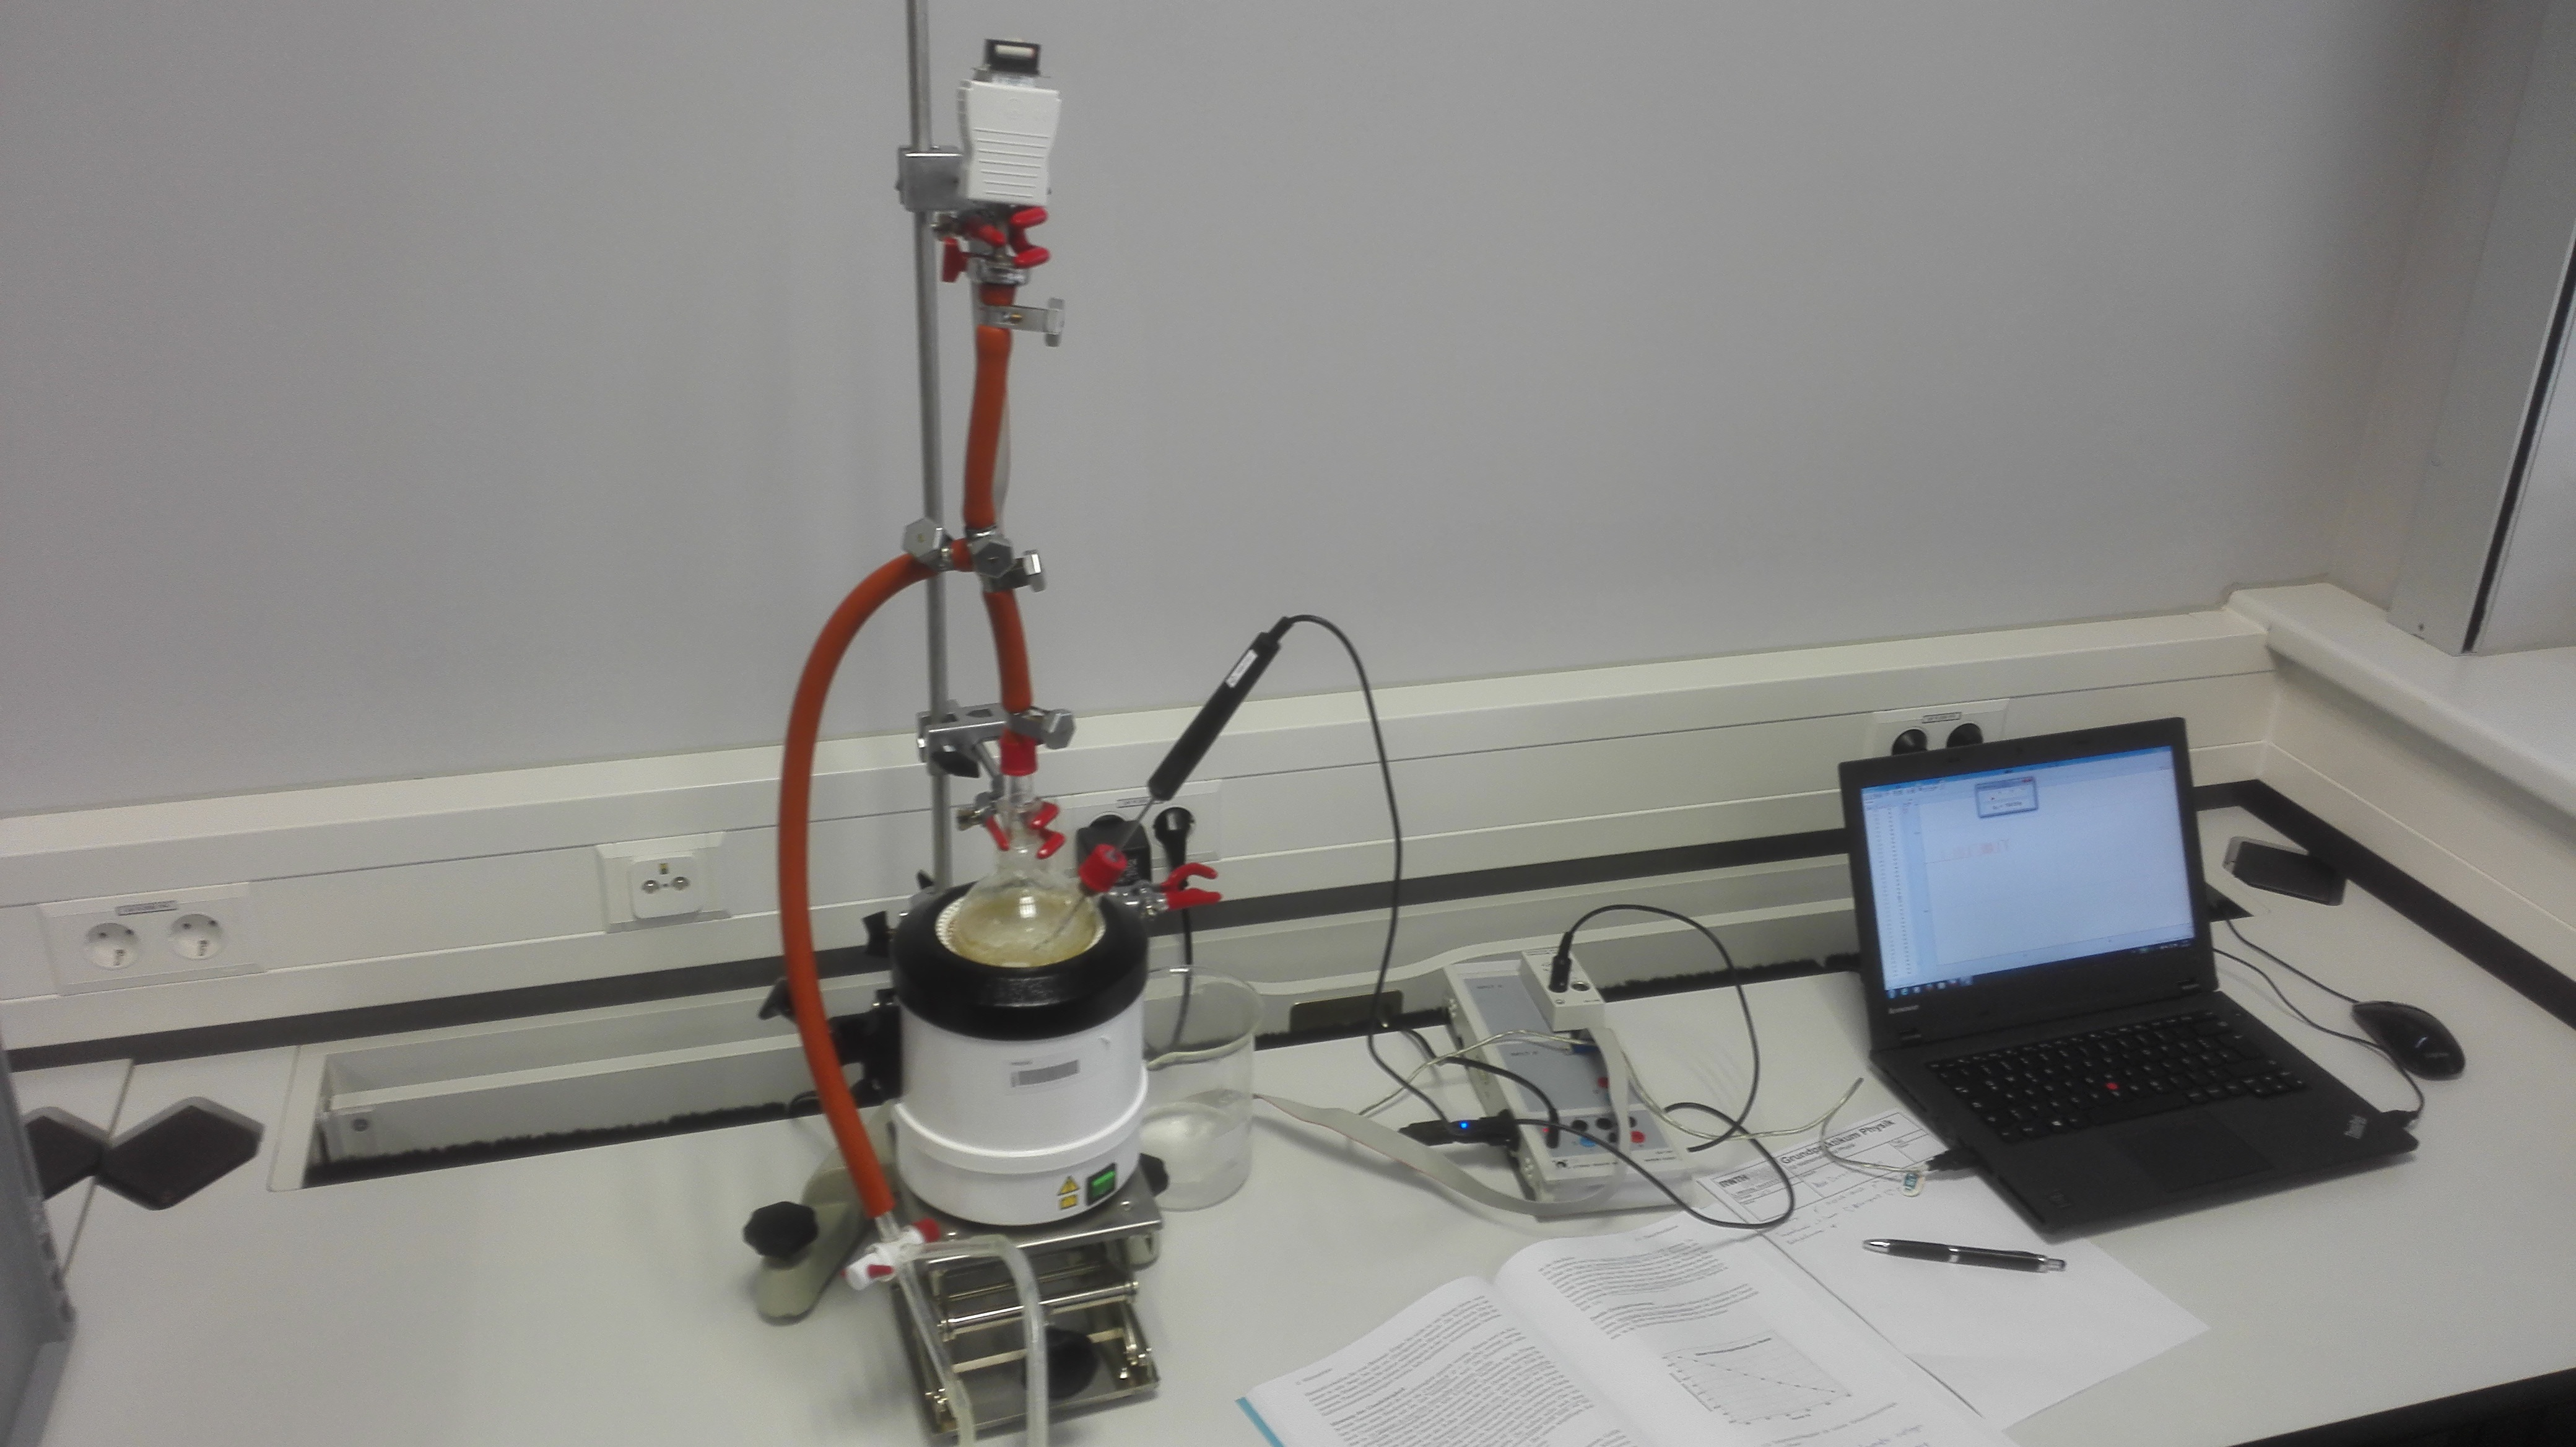
\includegraphics[width=\linewidth]{Bilder/AufbauB}
\caption[AufbauB]{Aufbau}
\label{fig:AufbauB}
\end{figure}

Der Aufbau ist in Abbildung \ref{fig:AufbauB} gezeigt. \\
Das Thermometer wird mit der Thermobox an das CASSY angeschlossen. Als Messbereich wird $-20C - 120C$ gewählt.\\
Der Druckmesser wird direkt an das CASSY angeschlossen und der Messbereich zu $0hPa - 1500hPa$ gewählt. Am CASSY werden Temperatur und Druck in Messintervallen von jeweils einer Sekunde gemessen. \\

Der Glaskolben wird etwa zur Hälfte mit Wasser gefüllt und über die entsprechenden Anschlüsse mit Temperaturfühler und Drucksensor verbunden. Sowohl der Kolben als auch die Messinstrumente werden am Stativ befestigt. Der Heizpilz wird auf dem ausgefahrenen Laborheber so unter den Kolben montiert, dass er schnell entfernt werden kann. Eine Handvakuumpumpe wird über den Dreiwegehahn mit dem Kolben verbunden.\\

Die Rauschmessung des Drucksensors wird zusammen mit der Kalibrierung des Temperaturfühlers durchgeführt. Dazu werden $300$ Messwerte aufgezeichnet.\\
Zur Überprüfung der Gasdichtigkeit wird mit der Handvakuumpumpe bei verschlossenem Auslass der Druck im Glaskolben unter $200hPa$ gesenkt und der zeitliche Verlauf des Drucks gemessen. Aus dem Anstieg des Druckes kann die Undichtigkeit des Aufbaus bestimmt werden. Der Druck sollte nach Möglichkeit mit weniger als $0,2 \dfrac{mbar}{min}$ steigen, um eine vernachlässigbare Undichtigkeit zu erzielen. \\

Im Hauptversuch wird bei geöffnetem Auslass das Wasser im Glaskolben bis zum Sieden erhitzt. Hat man sich davon überzeugt das der Kolben keine Luft mehr enthält wird der Auslass geschlossen, der Heizpilz entfernt und die Messung gestartet. Während des Abkühlens wird dann die Dampfdruckkurve aufgezeichnet bis das Wasser im Kolben aufhört zu sieden.\\
Am Ende des Messvorgangs lässt man das Wasser weiter bis auf Raumtemperatur abkühlen und führt gegebenenfalls eine zweite Dichtigkeitsmessung durch, um sich davon zu überzeugen, dass die Undichtigkeit des Aufbaus während des Versuchs nicht gestiegen ist. 

\section{Versuchsauswertung}






\end{document}